\chapter{Getting started}
\label{chptr:getting_started}

\section{Introduction}
\label{sect:introduction}
One of the first steps in computational simulations of continua is the specification of the domain, and its tessellation into non-overlapping cells or elements. In the context of computational ocean fluid dynamics, the domain is typically bound by \emph{open boundaries}, the \emph{free surface}, \emph{ocean floor} and perhaps an \emph{ice-shelf} as identified in figure \ref{fig:typical_ocean_modelling_domain}. In practice, domain boundaries are frequently extracted by topography/morphology data such as the data shown in figure \ref{fig:rtopo_atlas} for the region around the South Pole. The panels of figure \ref{fig:rtopo_atlas} show contour plots of a subset of the data available in the RTOPO dataset \citep{timmermann_et_al:2010}: The region bathymetry(left panel), surface elevation (right panel) and filled contours that characterise the surface of the region in terms of shelf-ice, sea or land.
\begin{figure}[htb!]\begin{center}
%\scalebox{0.6}{\includegraphics{}}
\caption[A typical domain encountered in computational ocean fluid dynamics.]{A typical domain encountered in computational ocean fluid dynamics.}
\label{fig:typical_ocean_modelling_domain}
\end{center}\end{figure}
\begin{figure}[htb!]\begin{center}
\scalebox{1.0}{\includegraphics{meshing_images/rtopo_maps.pdf}}
\caption[Data from the the R-TOPO Antarctica atlas.]{Three data-sets from the R-TOPO Antarctica atlas. Left: Bathymetry. Centre: Identification of surface cover. Right: surface elevation. All plots in stereographic projection}
\label{fig:rtopo_atlas}
\end{center}\end{figure}
\par
Usually the domain boundary specification can be essentially reduced to an operation in two-dimensions alone: The equations solved are two-dimensional (\eg the shallow-water equations) or, as is the case in \fluidity, the two dimensional mesh is projected to the top and bottom surfaces of the domain and a three-dimensional mesh is created during an \emph{``extrusion''} procedure, as conveyed in figure \ref{fig:2d_domain_and_extrusion}. Then the process of domain specification reduces to the specification of shorelines, grounding lines and open boundaries on a reference surface such that a closed domain is formed, as shown in figure \ref{fig:2d_domain_and_extrusion}. 
\begin{figure}[htb!]\begin{center}
%\scalebox{0.6}{\includegraphics{}}
\caption[A two dimensional mesh and schematic of the extrusion procedure.]{Left: A two-dimensional mesh. Right: Schematic conveying the extrusion procedure.}
\label{fig:2d_domain_and_extrusion}
\end{center}\end{figure}
\par
Another essential part of mesh generation for ocean modelling is the specification of mesh size. Smaller elements are typically required in shallow regions, near the coastlines (in order to accurately represent the aforementioned complex boundaries), in areas of steep bathymetry or simply in regions of interest (\eg tidal farm installations). Figure \ref{} shows the two-dimensional field of the mesh size metric as filled contours.
\par
It is clear from figures \ref{fig:typical_ocean_modelling_domain}, \ref{fig:2d_domain_and_extrusion} and \ref{fig:rtopo_atlas} that shorelines, grounding lines and the ocean floor are very complex: They are fractal-like geometries, characterised by a large range of scales. However, the extraction of boundaries and production of mesh size metric maps can be easily handled through \emph{Geographic Information Systems (GIS)} software. GIS software is capable of importing a large range or data-formats frequently used to represent morphology (\eg netCDF, png) or port \& coastline surveys (\eg shapefiles), such as shown in figure \ref{fig:rtopo_atlas}. Tools for processing such data are also provided, already facilitating some of the operations mentioned above.
Once the domain has been fully defined and the mesh size has been specified, this information can be passed to a mesh generator to produce the desired mesh. We have thus identified two essential components in a mesh generation procedure of ocean and coastal domains: First a component that can be used for processing of geographical information. Second a robust mesh generator. A typical work-flow in mesh generation of ocean and coastal domains is shown in figure \ref{fig:main_components}, showing the two aforementioned components. On the left side, the input data such as bathymetry is identified by the green ellipse. The red ellipse identifies the interaction with the user in order to extract and plot boundaries and the desired mesh-size metric. Note that the interaction of the user and the GIS software and the communication of information between the GIS software and the meshing software is accomplished through the \emph{meshing plug-ins}, the third component of the work-flow, and the subject of this manual.


\begin{figure}[htb!]\begin{center}
\scalebox{1.0}{\includegraphics{meshing_images/ocean_mesh_generation_overview.pdf}}
\caption[The usual meshing workflow.]{A work-flow typical in mesh generation of ocean and coastal domains.}
\label{fig:main_components}
\end{center}\end{figure}
\par
As figure \ref{fig:main_components} shows the software of choice is Quantum GIS and Gmsh:
\begin{enumerate}
  \item{\emph{Quantum GIS} (QGIS, \url{http://www.qgis.org/}):} is a user friendly Open Source Geographic Information System (GIS) licensed under the GNU General Public License. QGIS is an official project of the Open Source Geospatial Foundation (OSGeo). It runs on Linux, Unix, Mac OSX, Windows and Android and supports numerous vector, raster, and database formats and functionalities. A very attractive feature of QGIS is its extensibility via python ``plug-ins''. This method is used here to provide the interactions described above withthe help of figure \ref{fig:main_components} as a part of QGIS.
  \item{\emph{Gmsh} (\url{http://www.geuz.org/gmsh/}):gmsh licence and quick description}
\end{enumerate}
The remainder of this manual, bla bla bla....



\section{Obtaining and using Quantum GIS}
\label{sect:obtaining_and_using_qgis}

\subsection{Obtaining Quantum GIS}
\label{sec:install}
On the Ubuntu Linux distribution {Q}{G}{I}{S} is available through the Ubuntu package system and can be installed by typing: 

\begin{example}
\begin{lstlisting}[language=bash]
  wajig install qgis
\end{lstlisting}
\end{example}

To obtain useful supporting packages, add the UbuntuGIS repository,  see

\url{https://wiki.ubuntu.com/UbuntuGIS}.

This can be done with the following:

\begin{example}
  \begin{lstlisting}[language=bash]
  $ sudo add-apt-repository ppa:ubuntugis/ppa 
  $ wajig update
\end{lstlisting}
\end{example}

and install the following:

\begin{example}
  \begin{lstlisting}[language=bash]
  $ wajig install blender qgis python-shapely inkscape grass
    qgis-plugin-grass thuban gmt gpsbabel gpx2shp gpsd 
    gpsd-clients gpsdrive gpsman avce00 e00compr cgi-mapserver
    mapserver-bin perl-mapscript php5-mapscript python-mapscript
    postgis python-gdal proj libterralib1c2a
\end{lstlisting}
\end{example}

Note that on Precise, you need to replace the last library \emph{libterralib1c2a} with \emph{libterralib}.

\subsubsection{Direct Download}

To either use a newer version of the software or to simply gain access to
QGIS without installing the system's packages, a pre-compiled QGIS
client can be downloaded from the QGIS website at:

\url{http://hub.qgis.org/projects/quantum-gis/wiki/Download}

This download page has pre-compiled client software for 32-bit and 64-bit
Windows, Linux, and Mac OS X. Administrative privileges may be needed on the
computer to install the software.

\subsubsection{Supporting Packages}
In order for the \emph{Mesh NetCDF} and \emph{Define Boundary ID's} plugins to work, the Python package `Shapely' will need to be installed. This package carries out vector operations such as intersections when working with Shapefile polygon objects. This package is listed in the large install block in Section~\ref{sec:install}.

\subsection{Running QGIS}

On a Ubuntu system, QGIS can be run by typing 'qgis' into a
terminal. Note that when running it entirely locally it can be heavy on both CPU
and graphics card which in turn means it is heavy on battery life if
intensively used on a laptop.

On a Mac the QGIS application will probably have been put in the
Applications directory during the install procedure, and it can be run from
there.

No information is available about how to run QGIS in Windows. 

which should return something like:

\begin{example}
  \begin{lstlisting}[language=bash]
  $ which qgis
  /usr/bin/qgis
\end{lstlisting}
\end{example}

\subsection{Using QGIS}
% Drawing polygons.
% Difference operation.
% Extracting contour. GUI or Polygonize.
% Removing parts of the domain.

\subsection{Reading in data}

%See fig.~\ref{fig:multiple1} and also in particular fig.~\ref{fig:calc}.


\subsubsection{Opening files}

\subsubsection{Reading in fields}


\section{Obtaining and using Gmsh}
\label{sect:obtaining_and_using_gmsh}

\section{Obtaining the plugins}
\label{sect:obtaining_the_plugins}
Please download the qgis-plugins-meshing Ubuntu package which is available in the following PPA:

\begin{example}
  \begin{lstlisting}[language=bash]
  ppa:meshing/release
\end{lstlisting}
\end{example}

(which depends on packages in ppa:ubuntugis/ppa)

Commands required:
\begin{example}
  \begin{lstlisting}[language=bash]
  sudo add-apt-repository ppa:ubuntugis/ppa
  sudo add-apt-repository ppa:meshing/release
  sudo apt-get update
  sudo apt-get install qgis-plugins-meshing
\end{lstlisting}
\end{example}

If the final command fails, please download the package manually from
\url{http://amcg.ese.ic.ac.uk/~asc/public/qgis-plugins-meshing_1.9_all.deb}
and install with

\begin{example}
  \begin{lstlisting}[language=bash]
  sudo dpkg -i qgis-plugins-meshing_1.9_all.deb
\end{lstlisting}
\end{example}

(there is a fix for Precise, which is currently being processed by Launchpad).

